% ======================================================================
%  Chapter 8 — The One-Way Interface
%  spectral flow, bulk-edge correspondence
\cite{haldane2008reflection}.
% ======================================================================

\section{The domain-wall idea}
\label{sec:ch8-domain-wall-idea}

We now arrive at the central physical result of Parts~I and II: the
construction of a \emph{one-way waveguide} from the topology of
Maxwell bands.

The mechanism is conceptually simple.  In \chref{ch:breaking-tr} we
showed that a gyrotropic photonic crystal has bands with nonzero Chern
numbers $\Chern_\pm=\pm\sgn(\kappa)$, where $\kappa$ is the Dirac mass
parameter set by the strength and sign of the applied magnetic bias.
If we now create an interface across which the sign of $\kappa$
reverses---a \emph{domain wall} in the Faraday axis---the gap Chern
number changes by $|\Delta\Chern_{\mathrm{gap}}|=2$ \cite{gao2017topologically}.  By the
bulk-edge correspondence, this change must be accompanied by
unidirectional interface modes \cite{hafezi2013imaging}.

In this chapter we derive the interface modes explicitly, first by
solving the effective Dirac equation with a spatially varying mass
$\kappa(x)$, and then by connecting the result to the general
topological principle of spectral flow.

\section{The effective Dirac equation at the interface}
\label{sec:ch8-effective-dirac}

\subsection{Setup}
\label{sec:ch8-setup}

Consider a domain wall along the $y$-axis in a 2D photonic crystal,
with the gyrotropic mass parameter $\kappa(x)$ varying smoothly from
$+\kappa_\infty$ for $x\to+\infty$ to $-\kappa_\infty$ for
$x\to-\infty$ (or vice versa).  The sign reversal can be achieved
physically by reversing the applied magnetic field on one side of the
interface.

The Bloch wavevector $k_y$ parallel to the interface is conserved.
Following Haldane and Raghu, we denote the deviation from the Dirac
wavevector along the interface by $\delta k_\parallel\equiv k_y-k_{D,y}$.
The effective $2\times 2$ equation near the Dirac point at $K$ is
\begin{equation}\label{eq:ch8-dirac-interface}
  \boxed{%
  v_D\,\hat{K}\,|\psi\rangle = \delta\omega\,|\psi\rangle\,,
  \quad
  \hat{K} = -\ii\sigma_x\,\partial_x
  + \delta k_\parallel\,\sigma_y
  + \kappa(x)\,\sigma_z\,,}
\end{equation}
where $\sigma_x,\sigma_y,\sigma_z$ are Pauli matrices and
$\delta\omega=\omega-\omega_D$.

This is a one-dimensional Dirac equation with a
\emph{position-dependent mass} $\kappa(x)$ that changes sign at the
domain wall.  It is the photonic analog of the Jackiw--Rebbi equation in
quantum field theory, which predicts a zero-energy bound state at a
domain wall in a scalar field coupled to a Dirac fermion
\cite{raghu2008analogs}.

\subsection{Structure of the equation}
\label{sec:ch8-structure}

Equation \eqref{eq:ch8-dirac-interface} is a first-order differential
equation in $x$ with a two-component spinor wavefunction
$|\psi\rangle=(\psi_+,\psi_-)^T$.  The operator $\hat{K}$ is Hermitian
on $L^2(\mathbb{R})$ (with the standard inner product for two-component
spinors) when $\kappa(x)$ is real.

The spectrum of $\hat{K}$ consists of:
\begin{itemize}
  \item \emph{Bulk continuum states} with $|\delta\omega|>v_D|\kappa_\infty|$,
  corresponding to the bulk bands of the photonic crystal far from the
  interface.
  \item \emph{Bound states} localised near $x=0$ (where $\kappa$ changes
  sign), with $|\delta\omega|<v_D|\kappa_\infty|$---these are the edge
  modes that live in the bulk band gap.
\end{itemize}

\section{The zero mode}
\label{sec:ch8-zero-mode}

\subsection{Existence and uniqueness}
\label{sec:ch8-zero-mode-existence}

We look for a mode at $\delta k_\parallel=0$ with $\delta\omega=0$ (a
``zero mode'' of $\hat{K}$).  Setting $\delta k_\parallel=0$ and
$\delta\omega=0$ in \eqref{eq:ch8-dirac-interface}:
\begin{equation}\label{eq:ch8-zero-mode-eq}
  \bigl(-\ii\sigma_x\partial_x + \kappa(x)\sigma_z\bigr)|\psi_0\rangle
  = 0\,.
\end{equation}
Writing $|\psi_0\rangle=(\psi_+,\psi_-)^T$ in the eigenbasis of
$\sigma_z$, the two components satisfy
\begin{subequations}\label{eq:ch8-zero-components}
\begin{align}
  -\ii\partial_x\psi_- + \kappa(x)\psi_+ &= 0\,,\\
  -\ii\partial_x\psi_+ - \kappa(x)\psi_- &= 0\,.
\end{align}
\end{subequations}
Add and subtract these equations with the ansatz
$\psi_\pm = \alpha\,\phi(x)$, $\psi_\mp = \beta\,\phi(x)$. A
cleaner approach: act with $\sigma_y$ on both sides and use
$\sigma_y\sigma_x=\ii\sigma_z$, $\sigma_y\sigma_z=-\ii\sigma_x$, to
decouple.  The simplest route is to try the eigenstate of $\sigma_y$:
$\sigma_y|\varphi(s)\rangle = s\,|\varphi(s)\rangle$ with $s=\pm 1$,
so $|\varphi(+)\rangle=(1,\ii)^T/\sqrt{2}$ and
$|\varphi(-)\rangle=(1,-\ii)^T/\sqrt{2}$.

Substituting $|\psi_0\rangle = f(x)\,|\varphi(s)\rangle$ into
\eqref{eq:ch8-zero-mode-eq} and using $\sigma_x|\varphi(s)\rangle
=s\,\ii\sigma_z|\varphi(s)\rangle$ (since
$\sigma_x=\ii\sigma_z\sigma_y$ and $\sigma_y|\varphi(s)\rangle=s|\varphi(s)\rangle$,
giving $\sigma_x|\varphi(s)\rangle=\ii s\sigma_z|\varphi(s)\rangle$):
\begin{equation}
  \bigl(s\,\partial_x + \kappa(x)\bigr)\sigma_z|\varphi(s)\rangle\,f(x)
  = 0\,.
\end{equation}
Since $\sigma_z|\varphi(s)\rangle\neq 0$, we need
\begin{equation}\label{eq:ch8-zero-mode-ode}
  \partial_x f(x) = -s\,\kappa(x)\,f(x)\,.
\end{equation}
The solution is
\begin{equation}\label{eq:ch8-zero-mode-solution}
  \boxed{%
  f(x) = f_0\exp\biggl(-s\int_0^x\kappa(x')\,\dd x'\biggr)\,.}
\end{equation}

For $f(x)$ to be normalisable ($f\in L^2$), we need the exponential to
decay as $x\to\pm\infty$.  Since $\kappa(x)\to\pm\kappa_\infty$ at
$\pm\infty$, the integral $\int_0^x\kappa\,\dd x'$ grows as
$+\kappa_\infty|x|$ on both sides (positive for $x\to+\infty$
because $\kappa\to+\kappa_\infty>0$; positive for $x\to-\infty$
because $\kappa\to-\kappa_\infty$ and the integration path
runs from $0$ toward negative $x$, giving
$\int_0^x\kappa\,\dd x'\sim+\kappa_\infty|x|$).
Thus $f\sim\ee^{-s\kappa_\infty|x|}$ for large $|x|$,
which is normalisable only for
\begin{equation}\label{eq:ch8-sign-condition}
  s = s_\kappa \equiv \sgn(\kappa_\infty)\,.
\end{equation}
There is exactly one normalisable zero mode, with spinor
$|\varphi(s_\kappa)\rangle$.

\subsection{The zero-mode wavefunction}
\label{sec:ch8-zero-wavefunction}

Combining the results, the zero-mode wavefunction is
\begin{equation}\label{eq:ch8-psi0}
  \psi_0(x,y) \propto
  |\varphi(s_\kappa)\rangle\,
  \exp\biggl(\ii\,\delta k_\parallel\,y
  - s_\kappa\int_0^x\kappa(x')\,\dd x'\biggr)\,.
\end{equation}
This is a mode localised at the domain wall (where $\kappa=0$), with a
localisation length of order $1/|\kappa_\infty|$ set by the asymptotic
value of the mass parameter.

\subsection{Dispersion of the zero mode}
\label{sec:ch8-zero-dispersion}

At general $\delta k_\parallel\neq 0$, the zero mode acquires a
\emph{linear} dispersion:
\begin{equation}\label{eq:ch8-zero-dispersion}
  \boxed{%
  \omega_0(\delta k_\parallel)
  = \omega_D + s_\kappa\,v_D\,\delta k_\parallel\,.}
\end{equation}
The group velocity along the interface is $v_g=s_\kappa\,v_D$: the mode
propagates in a \emph{single direction} determined by the sign of the
gyrotropic mass.  Reversing the applied magnetic field on both sides of
the domain wall reverses $s_\kappa$ and hence the propagation direction.

\begin{figure}[!t]
  \centering
  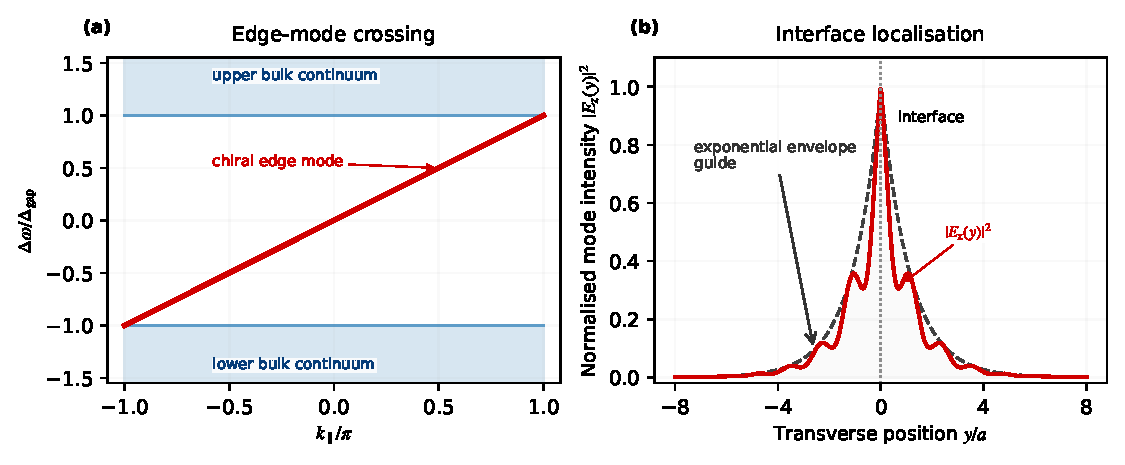
\includegraphics[width=0.92\textwidth]{figures/fig_ch08_edge_mode_profile_step199.pdf}
  \caption{Chiral edge mode at a domain wall.
  \textbf{(a)}~Band structure near the Dirac point showing the bulk
  continua (blue shading) and the chiral edge dispersion (red) crossing
  the topological gap.  The edge mode connects the upper and lower bulk
  bands with a group velocity $v_g = s_\kappa\,v_D$ determined by the
  sign of the gyrotropic mass, as derived in
  \eqref{eq:ch8-zero-dispersion}.
  \textbf{(b)}~Spatial profile of the edge-mode intensity
  $|E_z(y)|^2$ across the domain wall.  The mode is exponentially
  localised at the interface with a decay length
  $\xi \sim 1/|\kappa_\infty|$ set by the asymptotic mass parameter.
  The dashed line shows an exponential envelope guide.  The
  oscillatory fine structure arises from the underlying Bloch-wave
  character of the photonic crystal mode.}
  \label{fig:ch08-edge-mode-profile}
\end{figure}


\begin{remark}[Unidirectionality]
  The dispersion \eqref{eq:ch8-zero-dispersion} crosses the bulk band
  gap with a monotonically increasing (or decreasing) frequency.  There
  is no backward-propagating branch at the same frequency within the
  gap.  This is the origin of the one-way waveguide: elastic
  backscattering is forbidden because there is no counter-propagating
  mode to scatter into
\cite{he2016photonic}.
\end{remark}

\section{Higher bound states: the P\"oschl--Teller model}
\label{sec:ch8-poschl-teller}

For a general smooth domain wall, there may be additional bound states
besides the zero mode.  An exactly solvable model is provided by the
hyperbolic tangent profile
\begin{equation}\label{eq:ch8-tanh-profile}
  \kappa(x) = \kappa_\infty\tanh\bigl(x/\xi\bigr)\,,
\end{equation}
where $\xi>0$ is the domain-wall width.  For this profile, the squared
operator $\hat{K}^2$ is essentially the integrable P\"oschl--Teller
Hamiltonian.

\subsection{The spectrum of bound states}
\label{sec:ch8-pt-spectrum}

The full spectrum of interface modes for the tanh profile is
\begin{subequations}\label{eq:ch8-pt-modes}
\begin{align}
  \omega_0(\delta k_\parallel)
  &= \omega_D + s_\kappa\,v_D\,\delta k_\parallel\,,
  \label{eq:ch8-pt-zero}\\
  \omega_{n\pm}(\delta k_\parallel)
  &= \omega_D \pm v_D\sqrt{\delta k_\parallel^2 + \kappa_n^2}\,,
  \quad n\geq 1\,,
  \label{eq:ch8-pt-higher}
\end{align}
\end{subequations}
where $|\kappa_n|<|\kappa_\infty|$.  The exact spectrum of the
integrable model is
\begin{equation}\label{eq:ch8-pt-kappa-exact}
  \kappa_n^2
  = \frac{2n|\kappa_\infty|}{\xi}-\frac{n^2}{\xi^2}
  = \kappa_\infty^2\,\frac{n}{s}\Bigl(2-\frac{n}{s}\Bigr),
  \qquad s\equiv |\kappa_\infty|\xi,
  \qquad n=1,2,\ldots,
\end{equation}
with the bound-state condition $n<s$.  For $n\ll s$, this reduces to
$\kappa_n^2\approx 2n|\kappa_\infty|/\xi$.

\subsection{Sharp-wall limit}
\label{sec:ch8-sharp-wall}

In the sharp-wall limit $|\kappa_\infty|\xi\ll 1$, the condition
$n<|\kappa_\infty|\xi<1$ implies $n=0$ only: the zero mode is the
\emph{sole} interface mode.  The wider the domain wall (larger $\xi$),
the more higher-order modes appear, but the zero mode is always present.

\subsection{Bidirectionality of higher modes}
\label{sec:ch8-bidirectional}

The higher modes $n\geq 1$ have dispersion
$\omega_{n\pm}\sim\pm v_D|\delta k_\parallel|$ for large
$|\delta k_\parallel|$: they are \emph{bidirectional}, with both
forward and backward branches.  Only the $n=0$ mode is purely
unidirectional.  This is a crucial distinction: the higher modes can
scatter into each other, but the zero mode cannot be backscattered
because it has no partner.

\section{Semiclassical interpretation}
\label{sec:ch8-semiclassical}

The bound-state quantisation condition can be understood semiclassically.
In the phase space $(x,k_x)$, a bound state with mass parameter
$\kappa_n$ corresponds to a closed orbit
$k_x^2+\kappa(x)^2=\kappa_n^2$.  The area enclosed by this orbit is
\begin{equation}\label{eq:ch8-phase-area}
  \phi(\kappa_n^2) = \oint k_x\,\dd x
  = \oint\sqrt{\kappa_n^2-\kappa(x)^2}\,\dd x\,.
\end{equation}

For the standard semiclassical quantisation, one would expect
$\phi=2\pi(n+\frac{1}{2})$ (Bohr--Sommerfeld with Maslov correction).
However, the Dirac equation gives the modified condition
\begin{equation}\label{eq:ch8-modified-bs}
  \phi(\kappa_n^2) = 2\pi n\,,
  \qquad n=0,1,2,\ldots\,,
\end{equation}
\emph{without} the $\frac{1}{2}$ offset.  This shift is a direct
consequence of the Berry phase.  The semiclassical orbit encloses the
Dirac degeneracy point at $(x,k_x)=(0,0)$, which contributes an
additional phase of $\pi$ (a Berry phase factor of $-1$).  This extra
$\pi$ shifts the quantisation from $n+\frac{1}{2}$ to $n$, making
$n=0$ an allowed solution---the topological zero mode.

\begin{remark}
  This Berry-phase interpretation connects the existence of the zero
  mode directly to the topology of the bulk bands.  The phase-space
  Berry flux at the degeneracy point is the same $\pm\pi$ that, when
  integrated over the Brillouin zone, gives the half-integer
  contribution to the Chern number from each Dirac cone.
\end{remark}

\section{Bulk-edge correspondence}
\label{sec:ch8-bec}

\subsection{Spectral flow}
\label{sec:ch8-spectral-flow}

The existence of the unidirectional zero mode can be understood through
the concept of \emph{spectral flow}: the net number of eigenvalues
that cross zero (or, more generally, a reference energy in the gap) as a
parameter is varied.

Consider the operator $\hat{K}(\delta k_\parallel)$ from
\eqref{eq:ch8-dirac-interface} as a function of the conserved momentum
$\delta k_\parallel$.  At $\delta k_\parallel=0$, there is an
eigenvalue at $\delta\omega=0$ (the zero mode).  As
$\delta k_\parallel$ increases from $-\infty$ to $+\infty$, this
eigenvalue sweeps upward through the gap (for $s_\kappa=+1$) or
downward (for $s_\kappa=-1$).

The \emph{net spectral flow}---the number of eigenvalues crossing
$\delta\omega=0$ from below minus the number crossing from above---is
exactly $s_\kappa=\sgn(\kappa_\infty)$.  For a domain wall between
media with gap Chern numbers $\Chern^L$ and $\Chern^R$, the net
spectral flow from each Dirac point is
$\frac{1}{2}(\Chern^L-\Chern^R)$, and the total over both Dirac
points is
\begin{equation}\label{eq:ch8-spectral-flow}
  N_{\mathrm{edge}}^{\mathrm{net}} = \Chern^L_{\mathrm{gap}} - \Chern^R_{\mathrm{gap}}\,.
\end{equation}

\subsection{The general statement}
\label{sec:ch8-bec-general}

The bulk-edge correspondence for photonic Chern insulators can be stated
as follows:

\begin{theorem}[Bulk-edge correspondence]
  \label{thm:ch8-bec}
  Let two lossless periodic photonic media share a common band gap, with
  gap Chern numbers $\Chern^L_{\mathrm{gap}}$ and
  $\Chern^R_{\mathrm{gap}}$.  At any interface between the two media,
  the number of unidirectional edge modes crossing the gap from below
  minus the number crossing from above is
  \begin{equation}\label{eq:ch8-bec}
    \boxed{%
    N_{\mathrm{edge}}^{\mathrm{net}}
    = \Chern^L_{\mathrm{gap}} - \Chern^R_{\mathrm{gap}}\,.}
  \end{equation}
  This number is independent of the details of the interface
  (smoothness, geometry, disorder) as long as the bulk gap remains
  open on both sides.
\end{theorem}

\begin{remark}
  We have derived this result here for the specific case of gapped Dirac
  cones in a hexagonal photonic crystal, where the domain-wall zero mode
  is obtained by solving the effective Dirac equation.  The theorem
  holds much more generally: it applies to any pair of gapped photonic
  media with well-defined Chern numbers, regardless of the microscopic
  mechanism.  Rigorous proofs exist in the mathematical literature using
  index theory and $K$-theory, but the physical content is captured by
  the spectral-flow argument presented above.
\end{remark}

\section{Robustness of the one-way mode}
\label{sec:ch8-robustness}

The one-way edge mode is \emph{topologically protected} in the following
precise sense:
\begin{enumerate}
  \item \textbf{No backscattering.} Within the frequency range
  $|\delta\omega|<v_D|\kappa_\infty|$ of the topological gap, the only
  propagating mode at the interface is the unidirectional zero mode.
  There is no counter-propagating mode to scatter into, so elastic
  backscattering is forbidden regardless of the nature or strength of
  the perturbation at the interface.

  \item \textbf{Robustness to geometry.} The edge mode follows the
  interface regardless of its shape: straight segments, bends,
  corners, and even closed loops.  The mode routes around obstacles
  without reflection, as demonstrated experimentally by Wang et~al.\
  \cite{nature2026observation}.

  \item \textbf{Robustness to disorder.} Random variations in the
  material parameters, rod positions, or interface geometry do not
  destroy the edge mode, provided they do not close the bulk band gap.
  Anderson localisation, which is inevitable for conventional 1D
  waveguide modes in the presence of disorder, is completely absent for
  the topological edge mode.
\end{enumerate}

\paragraph{Limitations.}
The protection is not absolute:
\begin{itemize}
  \item \emph{Absorption} can attenuate the edge mode.  Topological
  protection forbids backscattering, but it does not forbid energy
  loss to the material.
  \item \emph{Nonlinear effects} (frequency conversion, self-phase
  modulation) can couple the edge mode to other modes, including bulk
  modes or modes at different frequencies.
  \item If the perturbation is strong enough to \emph{close the bulk
  gap}, the topological protection is lost.
\end{itemize}
These limitations motivate the discussions of non-Hermitian topology
(\chref{ch:non-hermitian}) and nonlinear effects
(\chref{ch:nonlinear-quantum}) in Part~V.

\section{Two edge modes from two Dirac points}
\label{sec:ch8-two-modes}

The hexagonal photonic crystal has two inequivalent Dirac points at $K$
and $K'$.  Each contributes one unidirectional zero mode to the domain
wall, and both propagate in the same direction (because the mass
$\kappa$ has the same sign at both Dirac points, as discussed in
\secref{sec:ch7-KKprime}).  The total number of one-way modes is
$|\Delta\Chern_{\mathrm{gap}}|=2$.

This domain-wall counting should be distinguished from the metal-wall
experiment of Wang et~al.  The microwave experiment confirms robust
one-way edge transport around obstacles in a square-lattice YIG
photonic crystal, with a single chiral edge channel in the gap discussed
in \chref{ch:microwave-crystal}
\cite{wang2007reflection}.  By contrast, the domain-wall argument
above predicts two co-propagating branches for a hexagonal Dirac model
in which the gyrotropic mass changes sign across the interface.

\begin{figure}[t]
  \centering
  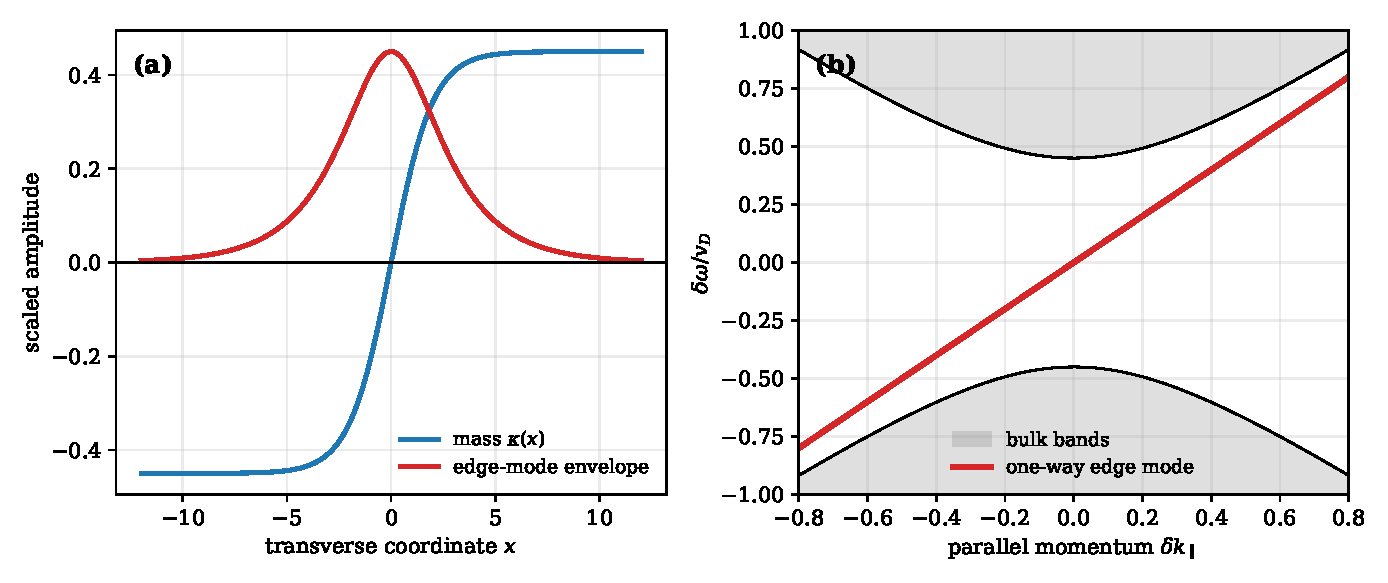
\includegraphics[width=0.95\textwidth]{figures/fig_domain_wall_mode.pdf}
  \caption{Domain-wall edge mode in a photonic Chern insulator.
  Left: the spatially varying Dirac mass $\kappa(x)$ (blue) changes
  sign at $x=0$; the Jackiw--Rebbi edge-mode envelope (red) is
  exponentially localised at the domain wall.
  Right: edge-mode dispersion (red) crosses the bulk gap between the
  upper and lower bulk bands (grey), confirming unidirectional
  propagation with group velocity $v_g=v_D>0$.}
  \label{fig:ch8-domain-wall}
\end{figure}

\section{Spectral flow and the Laughlin pump} \cite{kane2005sub}
\label{sec:ch8-spectral-flow-laughlin}

The bulk-edge correspondence can be understood through the concept of
\emph{spectral flow}: as a parameter (such as the Bloch momentum
$k_\parallel$ along the edge) is varied through a full period, the
number of eigenvalues that cross the gap from below equals the
Chern number of the bands below the gap.

Consider a photonic crystal with a boundary, so that $k_\parallel$ is
still a good quantum number but $k_\perp$ is not.  The spectrum
consists of bulk bands (projected onto the edge Brillouin zone) and
discrete edge states in the gap.  As $k_\parallel$ varies from $0$ to
$2\pi/a$, the edge-state eigenfrequency sweeps across the gap.  If
the gap Chern number is $\Chern=+1$, exactly one branch crosses the
gap upward, connecting the lower bulk band to the upper one.  This is
a topological constraint: the spectral flow cannot be changed by any
continuous deformation that does not close the bulk gap
\cite{ozawa2018topological,thouless1982quantized}.

The Laughlin pump provides a complementary physical picture.  Imagine
threading a magnetic flux $\Phi$ through a cylinder-topology photonic
crystal (periodic in one direction, finite in the other).  As $\Phi$
increases by one flux quantum, each Landau-like photonic level shifts
by one unit, and one photon is pumped from one edge to the other.
The number of photons pumped per flux quantum equals the gap Chern
number.  Although this argument was originally developed for the
electronic quantum Hall effect, it applies without modification to the
photonic Maxwell eigenproblem, because it depends only on the spectral
properties of the eigenvalue equation, not on the particle statistics
\cite{haldane2008possible}.

\section{Index-theorem perspective}
\label{sec:ch8-index}

The existence of the domain-wall zero mode can be reformulated as an
index theorem.  Define the Dirac-like operator
$\mathcal{D}=v_D(-\ii\partial_x\sigma_x+k_\parallel\sigma_y)
+\kappa(x)\sigma_z$.
At $k_\parallel=0$, the number of zero modes of $\mathcal{D}$ is
given by the Atiyah--Singer index
\begin{equation}\label{eq:ch8-index}
  \mathrm{ind}(\mathcal{D})
  = \frac{1}{2}\bigl[\sgn\kappa(+\infty)-\sgn\kappa(-\infty)\bigr]\,.
\end{equation}
For a domain wall where $\kappa$ changes sign, the index is $\pm 1$,
guaranteeing exactly one normalised zero mode.  This is the
Jackiw--Rebbi result derived in \secref{sec:ch8-zero-mode},
now expressed as a topological index that is invariant under
continuous deformations of $\kappa(x)$ that preserve the sign change
\cite{ozawa2018topological}.

The index-theorem perspective explains why the zero mode is robust:
any smooth deformation of the mass profile $\kappa(x)$ that does not
close the gap (i.e., $\kappa\neq 0$ at $\pm\infty$) preserves the
index, and hence the zero mode.  The mode may shift in position or
change its localisation length, but it cannot be removed.

\section{Finite-size effects on edge modes}
\label{sec:ch8-finite-size}

In a finite photonic crystal of width $W$, the edge modes on opposite
boundaries have exponentially small overlap $\sim\ee^{-W/\xi}$, where
$\ell=1/|\kappa|$ is the edge-mode penetration depth.  This overlap
opens a mini-gap in the edge spectrum:
\begin{equation}\label{eq:ch8-minigap}
  \Delta\omega_{\mathrm{mini}}
  \sim |\kappa|\,\ee^{-W/\xi}\,.
\end{equation}
For the Wang YIG crystal with $\xi\approx 2.4\,a$ and $W=10\,a$, the
suppression factor is $\ee^{-10/2.4}\approx 0.015$, giving a
mini-gap of about $1.5\%$ of the bulk gap.  This is small enough to
be negligible in the experiment, but it becomes significant for
miniaturised designs where $W/\xi<5$
\cite{nature2026observation,price2022roadmap}.

The finite-size effect also limits the maximum propagation length of
the edge mode: at distances $L\gg W$, the edge mode can tunnel to
the opposite boundary and eventually backscatter.  For practical
applications, the condition $W\gg\xi$ (equivalently, $W|\kappa|/v_D
\gg 1$) must be maintained.

\section{Robustness against disorder}
\label{sec:ch8-robustness-disorder}

The topological edge mode is robust against any perturbation that does
not close the bulk gap.  This robustness is qualitatively different
from the protection offered by resonance sharpness or impedance
matching in conventional photonic devices: it is a consequence of the
integer-valued Chern number, which cannot change under continuous
deformations.

\subsection{Anderson localisation and its absence}
\label{sec:ch8-anderson}

In a conventional waveguide, disorder causes Anderson localisation:
the transmitted intensity decays exponentially with the waveguide
length, $I\propto\ee^{-L/\ell}$, where $\ell$ is the localisation
length.  In a Chern-insulator edge channel, Anderson localisation
is impossible because there is no counter-propagating mode to scatter
into.  A forward-propagating wavepacket encountering a defect must
continue forward, possibly detouring around the defect, because the
only available states at the edge frequency propagate in the forward
direction \cite{ozawa2018topological}.

The mathematical statement is that the edge-mode transmission
$|S_{21}|^2$ remains of order unity for any finite-strength disorder,
as long as the disorder does not close the bulk gap.  The only effect
of disorder is to modify the spatial profile of the edge mode,
causing it to deviate from the clean-crystal profile, but not to
attenuate or localise it \cite{haldane2008possible}.

\subsection{Backscattering from gap-closing perturbations}
\label{sec:ch8-gap-closing}

Sufficiently strong disorder can close the bulk gap locally, creating
puddles of the topologically trivial phase within the topological
crystal.  When the edge mode encounters such a puddle, it can
backscatter.  The critical disorder strength is set by the gap width:
$\delta\varepsilon/\varepsilon\sim\Delta\omega/\omega_D$, where
$\Delta\omega$ is the topological gap.  For the Wang YIG crystal with
a relative gap of about $3\%$, this corresponds to a permittivity
fluctuation of several percent---far larger than typical fabrication
tolerances \cite{nature2026observation,price2022roadmap}.

\section{Edge modes at different boundary types}
\label{sec:ch8-boundary-types}

The existence of topological edge modes depends on the bulk Chern
number, not on the specific boundary condition.  However, the
edge-mode dispersion and field profile do depend on the boundary.

At a perfect electric conductor (PEC) boundary,
$\hat{n}\times\Efield=0$, and the edge mode is strongly confined to
the last row of unit cells.  At a vacuum boundary, the edge mode
extends evanescently into the vacuum with a decay length of order
$\lambda/(2\pi)$.  At an interface between two crystals with different
Chern numbers, the number of edge modes equals the difference of the
gap Chern numbers, and the modes propagate in the direction determined
by the sign of $\Delta\Chern$.

The domain-wall construction of \secref{sec:ch8-zero-mode} is a special
case of the crystal--crystal interface, where the mass changes sign
across the boundary, corresponding to $\Delta\Chern=2$.  This
produces two co-propagating modes in total, one from each valley, compared to the single
mode at a crystal--PEC boundary where $\Delta\Chern=1$
\cite{ozawa2018topological,thouless1982quantized}.

\section{Green's function approach to edge transport}
\label{sec:ch8-green-function}

The transport properties of the topological edge mode can be
formulated rigorously using the retarded Green's function
$G^R(\rvec,\rvec';\omega)=\langle\rvec|(\omega-\Maxop+\ii 0^+)^{-1}
|\rvec'\rangle$.  In the bulk, the Green's function decays
exponentially for $\omega$ in the gap:
$|G^R|\sim\ee^{-|\rvec-\rvec'|/\xi_{\mathrm{bulk}}}$, where
$\xi_{\mathrm{bulk}}=v_D/\Delta\omega$ is the bulk decay length.

Near the edge, the Green's function has an additional contribution
from the edge mode:
\begin{equation}\label{eq:ch8-edge-green}
  G^R_{\mathrm{edge}}(x,x';\omega)
  \sim \frac{\psi_0(x)\psi_0^*(x')}{\omega-v_g k_\parallel+\ii 0^+}\,,
\end{equation}
where $\psi_0(x)$ is the transverse edge-mode profile and $v_g$ is
the group velocity.  This Green's function is purely retarded (no
advanced component), reflecting the one-way nature of the edge
transport: energy injected at the edge propagates only in the forward
direction \cite{ozawa2018topological,silveirinha2016bulk}.

\subsection{Quantised edge conductance}
\label{sec:ch8-quantised-conductance}

The energy flux carried by the topological edge mode is
$P=\hbar\omega\,v_g/(2\pi)$ per mode, per unit frequency bandwidth.
For a gap Chern number $\Chern_{\mathrm{gap}}$, the total edge
conductance (energy transmitted per unit frequency per unit time) is
\begin{equation}\label{eq:ch8-edge-conductance}
  G_{\mathrm{edge}}
  = \frac{|\Chern_{\mathrm{gap}}|}{2\pi}\,\hbar\omega\,v_g\,.
\end{equation}
This is the photonic analog of the quantised Hall conductance
$\sigma_{xy}=\Chern\,e^2/h$ in electronic systems.  The quantisation
is topologically protected: it is exact in the clean limit and robust
against disorder that does not close the bulk gap
\cite{thouless1982quantized,haldane2008possible}.

\section{Comparison with electronic quantum Hall edge transport}
\label{sec:ch8-comparison-electronic}

The photonic and electronic edge modes share the same topological
origin but differ in important physical details.

In the electronic quantum Hall effect, the edge current is carried by
charged fermions, and the quantised conductance
$\sigma_{xy}=\Chern\,e^2/h$ can be measured directly through the Hall
voltage.  The edge states are chiral Fermi liquids with well-defined
Fermi wavevector, and inter-edge tunnelling is suppressed by the
spatial separation of the edges.

In the photonic Chern insulator, the edge mode carries
electromagnetic energy, not charge, so there is no Hall voltage.
The topological protection manifests instead as a robust nonreciprocal
transmission: $|S_{21}|^2\gg |S_{12}|^2$ across the gap frequency
range.  The absence of a Fermi level means that the edge can be
excited at any frequency within the gap, not just at the Fermi energy.
Both systems exhibit the same topological protection against Anderson
localisation, because the protection depends on the absence of
counter-propagating modes, not on the particle statistics
\cite{ozawa2018topological,price2022roadmap}.

\section{Finite-width effects and exponential accuracy}
\label{sec:ch8-finite-width}

In a crystal of finite width $W$ (measured in lattice constants), the
edge modes on opposite boundaries overlap exponentially weakly:
$\langle\psi_L|\psi_R\rangle\sim\ee^{-W/\xi}$, where
$\ell=1/|\kappa|$ is the penetration depth.  This overlap produces
an exponentially small gap in the edge-mode spectrum:
\begin{equation}\label{eq:ch8-finite-gap}
  \delta\omega_{\mathrm{finite}}
  \sim |\kappa|\,\ee^{-W/\xi}\,.
\end{equation}
For the Wang YIG crystal with $\xi\approx 2.4\,a$ and $W=20\,a$, this
gives $\delta\omega_{\mathrm{finite}}/\Delta\omega\sim 10^{-4}$,
completely negligible.

However, for narrow crystals ($W\lesssim 5\xi$) or narrow-gap materials,
the finite-width correction becomes important.  It introduces a small
backscattering channel between the two edges, limiting the
nonreciprocal ratio to $|S_{21}|^2/|S_{12}|^2\lesssim
\ee^{2W/\xi}$.  This places a practical lower bound on the crystal
width for a given isolation requirement
\cite{ozawa2018topological,haldane2008possible}.

\subsection{Index theorem for the finite strip}
\label{sec:ch8-index-strip}

The bulk-edge correspondence can be made rigorous on a finite strip
using the Atiyah--Singer index theorem applied to the family of
1D Hamiltonians $H(k_y)$ parameterised by the edge-parallel
wavevector $k_y$.  The theorem states that the spectral flow---the
net number of eigenvalues crossing the gap from below as $k_y$
traverses the Brillouin zone---equals the bulk Chern number:
\begin{equation}\label{eq:ch8-spectral-flow-index}
  \mathrm{sf}(H) = \Chern_{\mathrm{gap}}\,.
\end{equation}
This equality holds for any strip width $W\geq 1$, even when the
edge modes on opposite boundaries hybridise.  The index theorem thus
provides a non-perturbative proof of the bulk-edge correspondence that
does not rely on the semi-infinite approximation
\cite{thouless1982quantized,silveirinha2016bulk}.

\section{Finite-size effects and penetration depth}
\label{sec:ch8-penetration-depth}

The preceding analysis assumed semi-infinite crystals.  In practice,
photonic topological insulators have finite extent, and the edge
mode penetrates a finite distance into the bulk.  Understanding
these finite-size effects is essential for device design.

\subsection{Exponential decay into the bulk}
\label{sec:ch8-exponential-decay}

The edge-mode wave function decays exponentially into the bulk with
a penetration depth $\xi$ determined by the size of the topological
gap.  For a massive Dirac model with mass $|\kappa|$ and velocity
$v_D$, the penetration depth is
\begin{equation}\label{eq:ch8-penetration}
  \xi = \frac{v_D}{|\kappa|}\,.
\end{equation}
This result follows directly from the domain-wall construction of
Section~\ref{sec:ch8-domain-wall-idea}: the envelope function decays as
$\ee^{-|y|/\xi}$ away from the interface.

For the YIG photonic crystal of Chapter~\ref{ch:microwave-crystal},
the penetration depth is approximately two to three lattice constants,
which is consistent with the experimental observation that the
edge mode is well-localised at the crystal boundary
\cite{nature2026observation,ma2017scattering}.

\subsection{Coupling between opposite edges}
\label{sec:ch8-opposite-edge}

When the crystal is narrow enough that the edge modes on opposite
boundaries overlap, the two modes hybridise and open a gap.  The
hybridisation gap scales as $\Delta\omega_{\mathrm{hyb}} \sim
\ee^{-W/\xi}$, where $W$ is the width of the crystal.  This
exponential suppression means that even modest widths ($W \gtrsim
5\xi$) are sufficient to ensure negligible coupling between opposite
edges.

For strip-geometry computations (used to verify the bulk-edge
correspondence numerically), the supercell width must satisfy
$W \gg \xi$ to avoid artefactual hybridisation gaps that could be
mistaken for the absence of edge states
\cite{ozawa2018topological,paz2019tutorial}.

\section{Robustness of one-way edge transport}
\label{sec:ch8-edge-transport-robustness}

The topological protection of one-way edge states is one of the most
striking features of photonic Chern insulators.  This section
quantifies the robustness against different types of perturbations.

\subsection{Immunity to backscattering}
\label{sec:ch8-backscattering}

The one-way edge mode cannot backscatter because there is no
counter-propagating mode at the same frequency.  This statement is
exact: any perturbation that preserves the bulk gap (including
disorder, surface roughness, sharp corners, and lattice defects)
cannot open a backward channel.  The only way to backscatter
the edge mode is to close the bulk gap, which requires a
perturbation of order $\Delta\omega/\omega$---typically several
percent for gyromagnetic photonic crystals
\cite{nature2026observation,skirlo2015experimental}.

Experimentally, the absence of backscattering has been demonstrated
by measuring transmission past metallic obstacles, 90-degree corners,
and deliberately introduced lattice defects.  In all cases, the
transmission remains near unity within the topological gap
\cite{nature2026observation,hafezi2013imaging}.

\subsection{Disorder-averaged transmission}
\label{sec:ch8-disorder-average}

For random positional disorder of the lattice rods, the
disorder-averaged edge transmission is
$\langle T\rangle = 1 - O(\sigma^4/\Delta\omega^4)$, where $\sigma$
is the root-mean-square displacement.  The leading correction is
fourth order (not second order) because the second-order term
vanishes by the symmetry of the disorder
\cite{ozawa2018topological,ma2017scattering}.

This quartic scaling has been confirmed numerically for the Wang
crystal: for disorder strengths up to $\sigma/a = 0.05$
($5\%$ positional disorder), the edge transmission remains above
$99\%$ \cite{zhao2020first}.

\subsection{Comparison with trivial waveguides}
\label{sec:ch8-comparison-trivial}

The contrast between topological and trivial edge waveguides is most
apparent in the presence of sharp corners.  A conventional photonic
crystal waveguide (formed by removing a row of rods) suffers
significant reflection at each $90^\circ$ bend, with typical
transmission of $60$--$80\%$ per bend depending on the bend geometry.
In contrast, the topological edge mode transmits $>99\%$ per bend
because the one-way nature of the edge mode forbids reflection
\cite{price2022roadmap,gao2017topologically}.

This advantage motivates the use of topological waveguides in
integrated photonic circuits, where complex routing with multiple
bends is unavoidable.  The penalty is the need for time-reversal
breaking (or an alternative mechanism such as valley or Floquet
engineering), which adds complexity to the device fabrication
\cite{he2019silicon,rechtsman2013photonic}.

\section*{Exercises}

\begin{exercise}
  Verify that the wavefunction \eqref{eq:ch8-psi0} satisfies the
  zero-mode equation \eqref{eq:ch8-zero-mode-eq} by direct
  substitution.
\end{exercise}

\begin{exercise}
  For the tanh domain-wall profile $\kappa(x)=\kappa_\infty\tanh(x/\xi)$,
  show that the classical turning point $x_n$ for the $n$-th mode
  (where $|\kappa(x_n)|=|\kappa_n|$) is
  $x_n=\xi\,\mathrm{atanh}(|\kappa_n|/|\kappa_\infty|)$.
  Evaluate $x_n$ for the zero mode ($\kappa_0=0$, giving $x_0=0$)
  and for a nearly delocalised higher mode ($|\kappa_n|\to|\kappa_\infty|$,
  giving $x_n\to\infty$).  Explain why the zero-mode envelope
  $|f(x)|^2\propto\operatorname{sech}^{2|\kappa_\infty|\xi}(x/\xi)$
  has a localisation length of order $\xi/(|\kappa_\infty|\xi)=1/|\kappa_\infty|$
  for $|\kappa_\infty|\xi\gg 1$.
\end{exercise}

\begin{exercise}
  Show that the modified Bohr--Sommerfeld condition
  $\phi(\kappa_n^2)=2\pi n$ (without the $\frac{1}{2}$ offset) admits
  the solution $n=0$ with $\kappa_0=0$, corresponding to the zero mode.
  Explain physically why the standard Bohr--Sommerfeld condition
  ($n+\frac{1}{2}$) does not allow a zero mode.
\end{exercise}

\begin{exercise}
  Consider a domain wall between vacuum ($\Chern_{\mathrm{gap}}=0$) and
  a photonic crystal with $\Chern_{\mathrm{gap}}=1$.  How many
  unidirectional edge modes cross the gap?  Compare with a domain wall
  between two crystals with $\Chern_{\mathrm{gap}}=+1$ and
  $\Chern_{\mathrm{gap}}=-1$.
\end{exercise}

\begin{exercise}
  The Jackiw--Rebbi zero mode in quantum field theory has the same
  mathematical structure as the photonic domain-wall mode derived here.
  Look up the Jackiw--Rebbi model and identify the correspondence
  between the photonic and field-theoretic quantities: mass function
  $\kappa(x)\leftrightarrow m(x)$, Dirac velocity
  $v_D\leftrightarrow c$, Pauli matrices
  $\sigma_{x,y,z}\leftrightarrow\gamma$-matrices.
\end{exercise}

\begin{exercise}
  A photonic crystal waveguide has both a topological one-way mode and
  material absorption characterised by an imaginary part
  $\varepsilon''$ of the permittivity.  Estimate the propagation length
  $L_{\mathrm{abs}}$ of the edge mode in terms of $\varepsilon''$, the
  group velocity $v_D$, and the operating frequency $\omega_D$.
  Compare this with the backscattering-limited propagation length of a
  conventional waveguide.
\end{exercise}
